\section{Struktur der Diplomarbeit}
\setauthor{Felix Dumfarth}

Die folgenden Themengebiete wurden in der Diplomarbeit abgewickelt:

\textbf{Technischer Hintergrund}: Im technischen Hintergrund geht es um notwendiges Vorabwissen über maschinelles Lernen und damit verbunde Themengebiete wie Deep Learning und neuronale Netze, deren Verständnis relevant für die darauffolgenden Themengebiete ist.

\textbf{Toolstack}: Der Toolstack präsentiert die verwendeten Tools und Technologien, die zur Erstellung der Diplomarbeit genutzt wurden.

\textbf{Chatbots am Beispiel Rasa}: Dieses Kapitel beschreibt die Komponenten und die Entwicklung eines Chatbots mit Rasa im Detail.

\textbf{Implementierung}: Dieses Kapitel handelt von der Entwicklung und der Umsetzung des Chatbots und seinen Begleitprodukten aus dem praktischen Teil der Diplomarbeit.

\textbf{Evaluation}: Die Evaluation gibt einen Überblick über die Ergebnisse der Arbeit und, welche Ziele erfüllt wurden.



\section{Ausgangslage}
\setauthor{Felix Dumfarth}

Zahlreiche Organisationen bauen heutzutage auf eine starke Webpräsenz und wickeln dabei komplexe Produkt\- oder Leistungsfunktionalitäten ab.
Eine wichtige Rolle spielt dabei nicht nur der Kundenservice, sondern auch die Kommunikation, denn die Nutzer erwarten eine möglichst zeitnahe Beratung.
Die Bereitstellung von solchen Services ist derzeit immer noch mit sehr hohen Kosten verbunden.

\section{Istzustand}
\setauthor{Felix Dumfarth}
Es gibt viele Personen, die an dem Ausbildungsangebot der HTL Leonding interessiert sind und sich gerne schnell über die Schule informieren wollen.


\section{Problemstellung}
\setauthor{Felix Dumfarth}
Die HTL Leonding hat ein großes Informationsangebot, zu diesem gibt es viele Zugänge.
Dabei ist es zum Beispiel auf der Website oft schwierig den Überblick zu bewahren mit den vielen Unterseiten und daher wäre eine Unterstützung zum Finden für die vielen Informationen hilfreich.

\section{Aufgabenstellung}
\setauthor{Felix Dumfarth}
In dieser vorliegenden Arbeit soll ein Chatbot für die HTL Leonding Website erstellt werden, der Besucherinnen und Besuchern einfach und schnell schulspezifische Fragen beantworten soll.
Jedoch soll es auch möglich sein, dass der Bot auch als Grundlage für weitere Arbeiten in der Schule, wie zum Beispiel der 3-D-Leonie, zum Einsatz kommen kann.

\section{Use-Cases}
\setauthor{Felix Dumfarth}

\begin{figure}[hbt!]
    \centering
    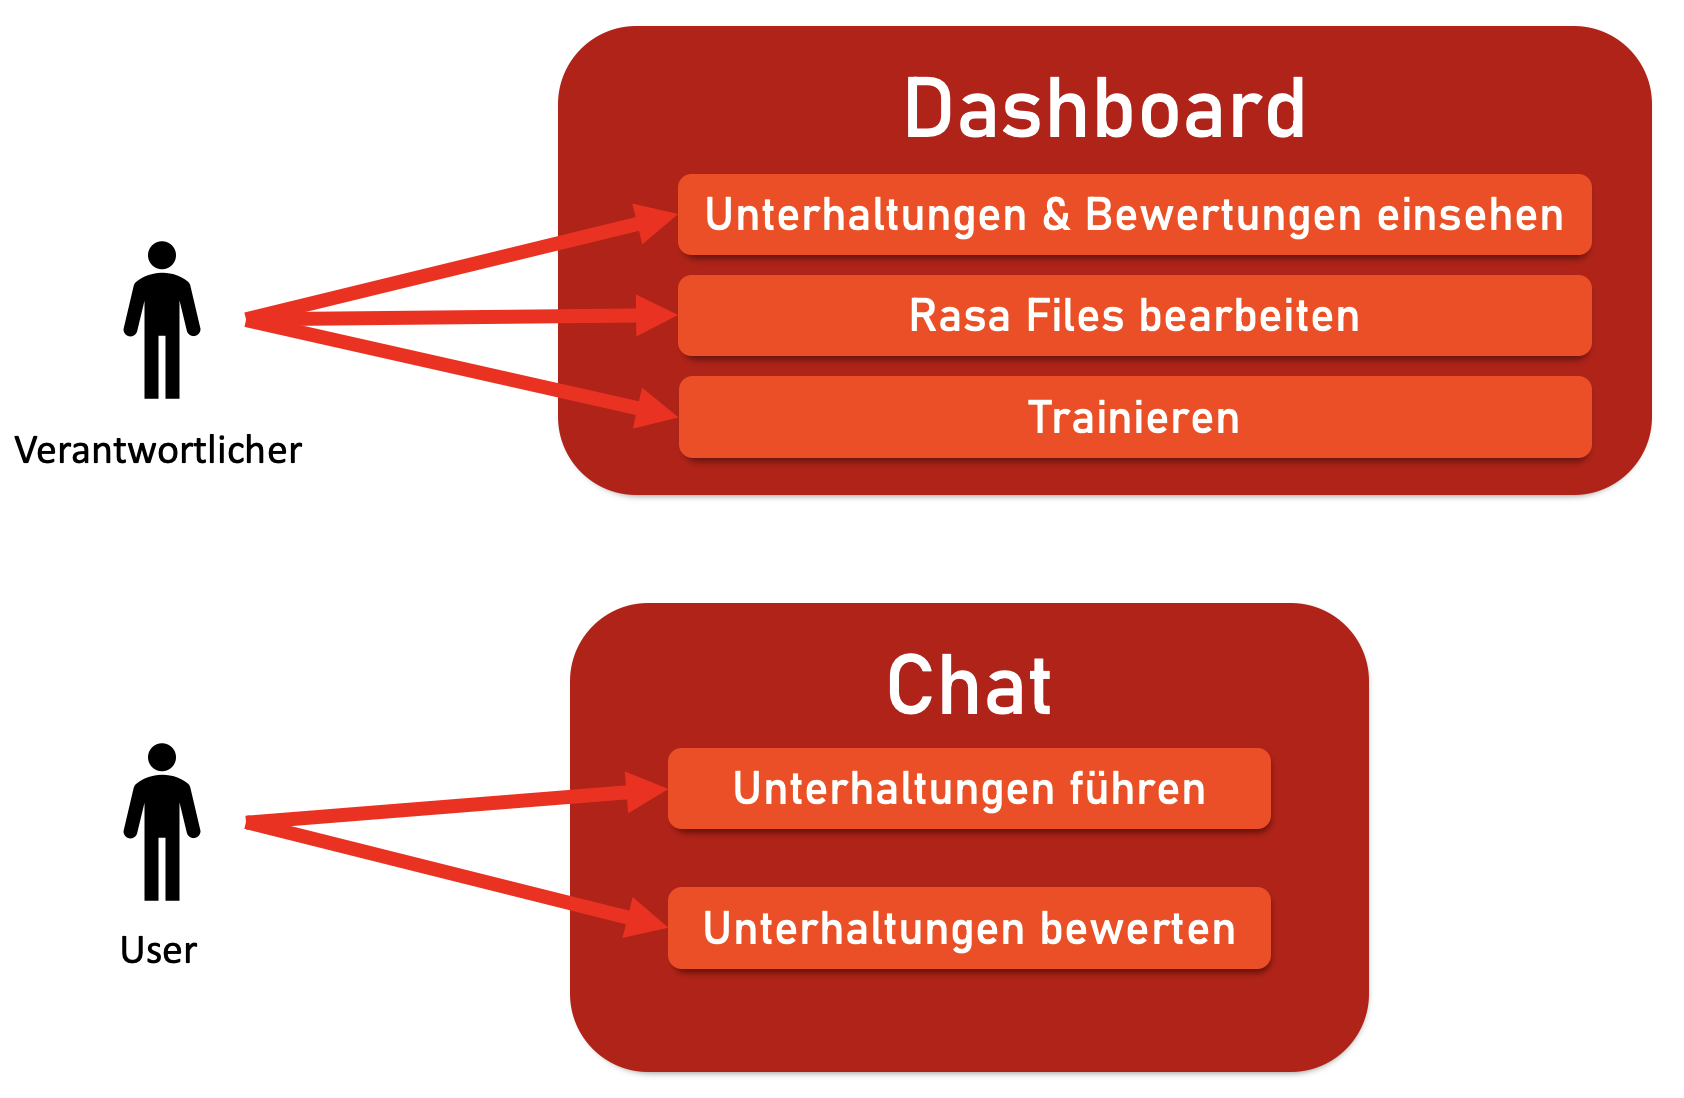
\includegraphics[scale=0.5]{pics/usecase}
    \caption{Use-Case Diagramm}
    \label{fig:impl:usecase}
\end{figure}

Der User kann hauptsächlich schulspezifische Unterhaltungen mit dem Chatbot führen und diese Unterhaltung anhand ihrer Qualität bewerten.
Aber auch generelle Informationen zum Bot, zu Rasa und Small Talk können bearbeitet werden.
Eine verantwortliche Person kann sich die Unterhaltungen und Bewertungen von Usern ansehen, sodass diese beurteilt werden können.
Außerdem kann die verantwortliche Person die Rasa Files \texttt{nlu.yml}, \texttt{stories.yml}, \texttt{rules.yml} und \texttt{domain.yml} bearbeiten und den Chatbot auffordern, sein neu erlerntes Wissen einzutrainieren.
